\documentclass[tikz]{standalone}
\usepackage{tikz,amsmath}
\usetikzlibrary{calc}
\tikzstyle{vertex} = [draw, shape=circle, minimum width=.3cm, inner sep=.5pt]
\begin{document}
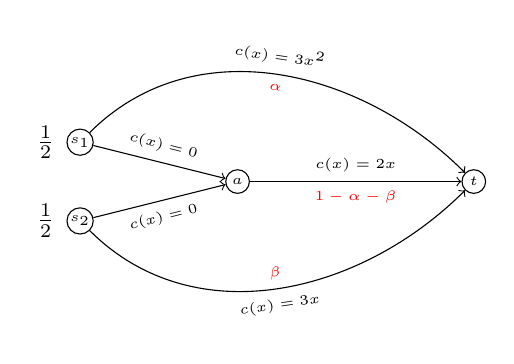
\begin{tikzpicture}[sloped]
    \draw (0,0) node[vertex] (s2) {\tiny{$s_2$}};
    \draw (0,1) node[vertex] (s1) {\tiny{$s_1$}};
    \draw (2,.5) node[vertex] (m1) {\tiny{$a$}};
    \draw (5,.5) node[vertex] (t) {\tiny{$t$}};
    \draw [->] (s1) -- node [above] {\tiny{$c(x)=0$}} (m1);
    \draw [->] (s2) -- node [below] {\tiny{$c(x)=0$}} (m1);
    \draw [->] (m1) -- node [above] {\tiny{$c(x)=2x$}} node [below,red] {\tiny{$1-\alpha-\beta$}} (t);
    \draw (s2) edge[out=-45,in=-135,->] node [below] {\tiny{$c(x)=3x$}} node [above,red] {\tiny$\beta$} (t);
    \draw (s1) edge[out=45,in=135,->] node [above] {\tiny{$c(x)=3x^2$}} node [below,red] {\tiny$\alpha$} (t);
    \node at (s1) [left=.2cm] {$\tiny{\frac{1}{2}}$};
    \node at (s2) [left=.2cm] {$\tiny{\frac{1}{2}}$};
\end{tikzpicture}
\end{document}
